\documentclass[11pt]{report}
\usepackage{standalone}
\graphicspath{ {images/} }
\setcounter{tocdepth}{5}
\setcounter{secnumdepth}{5}
\usepackage{natbib}
\usepackage{bibentry}
\bibliographystyle{agsm}
\usepackage{etoolbox}
\setlength{\parindent}{0em}
\setlength{\parskip}{0.25em}
\usepackage[raggedright]{titlesec}
\usepackage{hyperref}
\usepackage{capt-of}
\patchcmd{\bibliography}{\section*}{\section}{}{}
\titlespacing*{\chapter}{0pt}{-40pt}{10pt}
\titleformat{\chapter}[block]{\normalfont\huge\bfseries}{\thechapter}{15pt}{}
\usepackage{rotating}
\usepackage[titletoc]{appendix}
\usepackage{pgfgantt}
\usepackage{graphicx, rotating, caption, lscape, threeparttable}% \usepackage{amsmath}
\usepackage{array}
\usepackage{pdflscape}
\usepackage{geometry}
\usepackage{listings}
\usepackage[T1]{fontenc}
\usepackage[bottom]{footmisc}
\usepackage{subcaption}
\usepackage{float}




\begin{document}
\chapter{Discussion}

\section{Findings}

\subsection*{Quality of Data}
As the System collects its own data for classification it is worth reviewing the quality of this input data. Initially the System was going to be designed with a fully fledged Twitter API but due to the constraints of limited backdating of Twitters' tweets the historic HTML scraper of GetOldTweet's python was integrated. HTML scraping is subject to problems of rate-limiting, malformed scraping and document object model changes. Unfortunately, during the development of the System all of these problems occurred. Rate-limiting of the HTML scraping occurred early within data collection delaying progress for forming the dataset. Some of the returned tweets were also found to be malformed, specifically tweets with URL's as the URL was being incorrectly parsed from the HTML document object model (DOM). Finally, the historic scraper during the backdating of tweets became subject to a change in twitter's HTML DOM structure of the page causing unexpected behaviour within the running of the scraper. As a counter measure, a fix was implemented for this and was even integrated into the git repository of the scraper for the open source community to benefit from the fix also \footnote{Open Source contribution accessible via https://github.com/Jefferson-Henrique/GetOldTweets-python/commit/b9d5a1d21256832ceba797ab8b8b421e8572618a}.
\\

Towards the end of the development of the System the real-time scraper Tweepy was also integrated into the System. The System now had two sources of tweet data and the differences between the api's became apparent. Tweepy provided consistently more tweets, with a large amount of those tweets being retweets (\textit{tweets that are reposted and prefixed with RT}). These extra retweets all seemed to be truncated with `...' where the length of the retweet is too long. These points although small can effect the overall classification of a tweet, and thus is worth noting when comparing analysis computed by the system prior to the integration of Tweepy.
\\

Despite notions of inefficiency in data collection, both the historic and real-time scrapers were successfully integrated into the final System. The result of such integrations has allowed the System to collect a vast amount of data (see Table \ref{table:tweet-stats} for overall statistics) with the produced dataset having prospect of being made publicly available for others to use (after the publishing of this report).
\\
\vspace{-0.5cm}
\enlargethispage{\baselineskip}

\begin{center}
\begin{tabular}{ |p{2cm}||p{2cm}|}
 \hline
 Tweets & Users\\
 \hline
 7,110,544 & 1,210,824 \\
 \hline
\end{tabular}
\captionof{table}{Tweet Collection Statistics \textbf{as of publishing date}}
\label{table:tweet-stats}
\end{center}
\clearpage

\subsection*{Quality of Classifications}

Despite the large amount of data being collected from the brexit hashtags, the amount of training data available to the classifiers was a small proportion. The decision was also taken to improve the classification accuracy by exempting tweets containing malformed URL's (i.e. URL's that could not be replaced via a regular-expression) and tweets containing images from the classification process as it could be argued to be harder to extract sentiment from these tweets. Therefore, the small proportion training set became even smaller from the exemption of tweets. The Naive Brexit Model still achieved a noteworthy average accuracy of 70\% however the Sentiment Model wasn't as accurate; only achieving 66\% somewhat responsible to it's weaker and smaller training set of 6096 tweets compared to the 22,120 tweets of the Naive Brexit Model. Bootstrapping an existing labelled tweet dataset for training the sentiment model was also an option however the preference of domain training data over generalized was chosen instead. 
\\

The classifications computed by the Naive Brexit model performed well on clear cut distinctions that encouraged or discouraged ``Britain leaving the European Union'' which can be seen in the correctly classified Brexit tweet section of Appendix A. Tweets which discussed being `out' or talked in the tense of having `left' were correctly classified as discussing leave. Where Tweets that discussed remaining or discussed leave associated phrases with a negative tone were classified as remain. However tweets which were sarcastic led to inaccurate classifications like the tweet in incorrectly classified Brexit tweets section of Appendix A. Neutral tweets also existed such as news stories and count down timers for Brexit commencement so these were misclassified as they didn't really belong to either of the classes which makes the case for whether the model should have been trained as a multinomial classifier containing a neutral classification rather than a binomial. Tweet's of a limited length also proved a problem to classification, ``Die hard \#Brexit'' only provides two words for classification after tokenization (removal of the hashtag) and thus the confidence in classification of this tweet was just over random distribution at 50.001\%
\\

The Sentiment model classifications performed well on tweets that were assertive or pessimistic towards ``Britain leaving the European Union'' which can be seen in the correctly classified Sentiment tweet section of Appendix A. Tweets that mentioned `regret' or condemned past and future events regarding brexit were correctly classified as being negative. Where Tweets that were humorous or contained assertive support tended to be classified correctly as positive. Again the same neutrality occurs this time in the overall emotion of the tweet is (see Incorrectly Classified Sentiment Tweets in Appendix A). Tweets which gave connotations of both classes were also incorrectly classified e.g. the same tweet contained the phrase ``A Huge Thank you to everyone for their superb and supportive'' and ``we must fight'' but was classified as negative despite the overall tone being narrowly more positive.
\\

Tweets outside of the topic of discussion were also collected, the likes of the recent American Presidential Elections adopted the hashtag ``\#StrongerTogether'' and various tweets had the Systems Brexit defined hashtags with content that was not at all related to the hashtags (see Offf Discussion Topic Tweets in Appendix A). The result of classifying these irrelevant tweets is the skew of overall classification statistics and is worth noting. It was due to the observation of changing use of hashtags that a very specific and limited subset of hashtags were actually used in formulating the training set of the Naive Brexit Model.

\subsection*{Test Coverage}
Due to time constraints within the project and complexity of various technologies, there is testing missing from some classes that entail spinning off new threads and thus prove harder to test. These classes such as the \texttt{BatchClassificationService} class have however been tested manually and walked through via an Django debugger to verify behaviour.


\subsection*{Results}
The results of the analysis found that volume of leave tweets (blue) was consistently higher than the volume of remain tweets (red) and the volume of positive tweets (green) was also consistently higher than negative ones (red). (see Figures \ref{fig:naive-results}, \ref{fig:brexit-results} and \ref{fig:sentiment-results} ). 
\\

\textit{N.B. all of the model result figures below were extracted from the System's website}

\begin{figure}[H]
        \begin{subfigure}[b]{0.33\textwidth}
                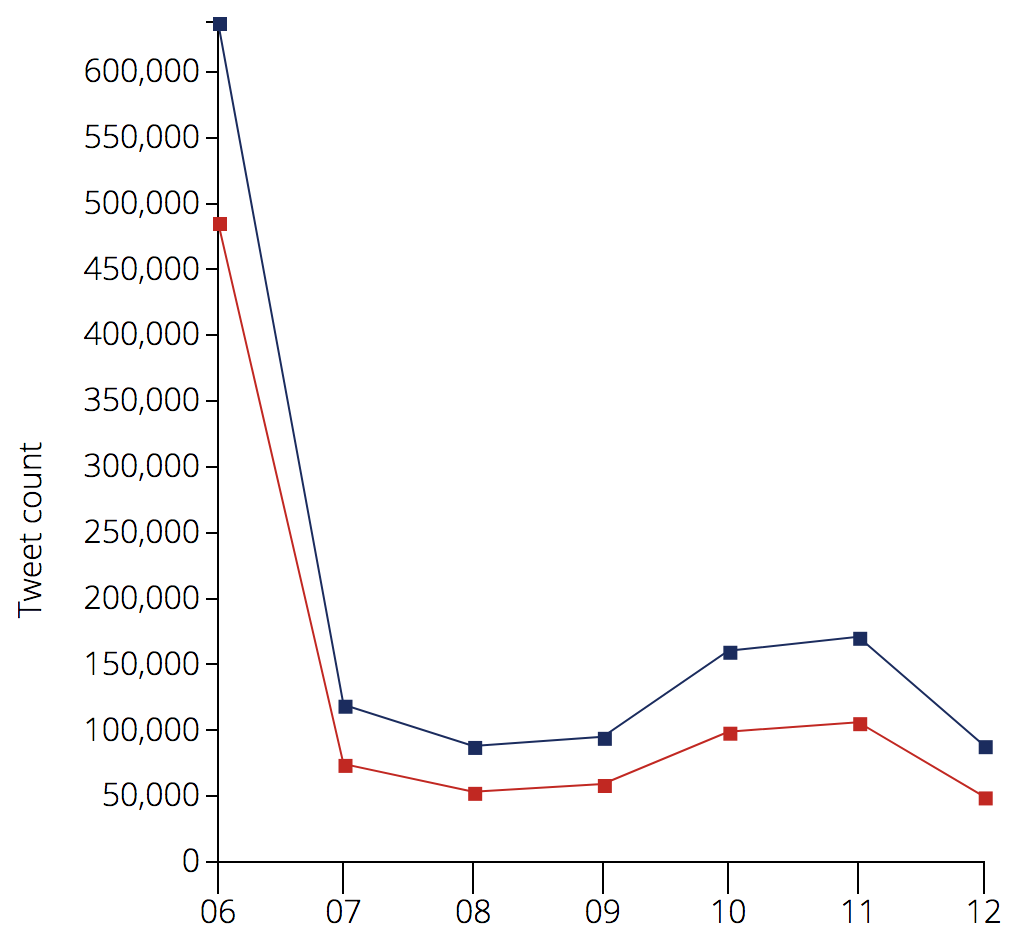
\includegraphics[width=\linewidth]{images/2016-naive.png}
                \caption{2016}
                \label{fig:gull}
        \end{subfigure}%
        \begin{subfigure}[b]{0.33\textwidth}
                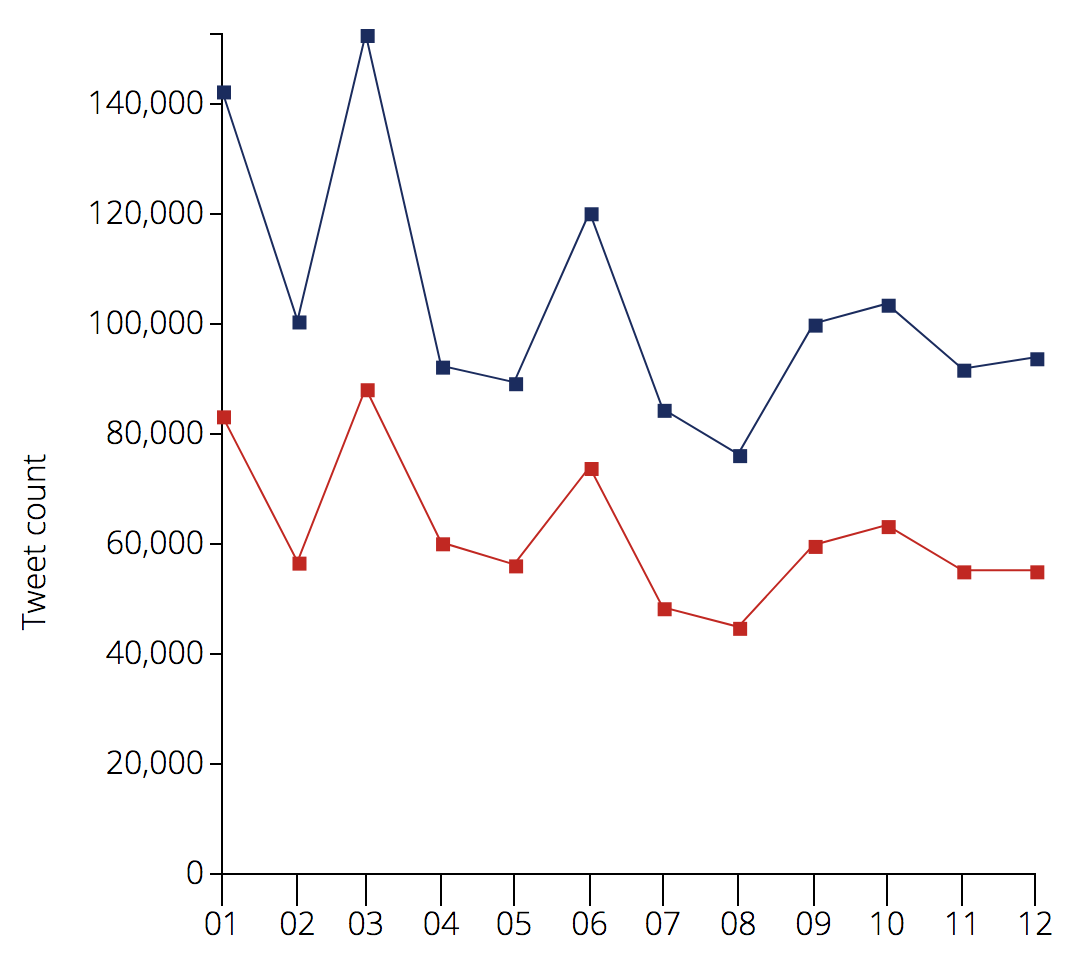
\includegraphics[width=\linewidth]{images/2017-naive.png}
                \caption{2017}
                \label{fig:gull2}
        \end{subfigure}%
        \begin{subfigure}[b]{0.30\textwidth}
                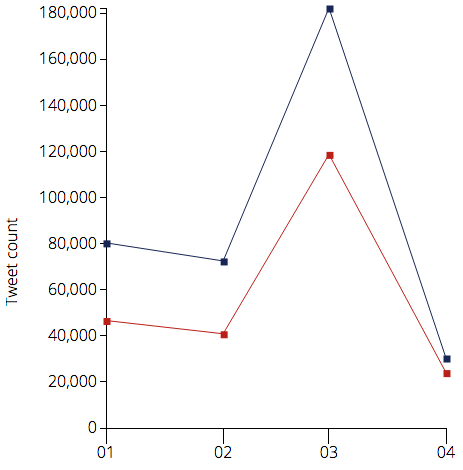
\includegraphics[width=\linewidth]{images/2018-naive.png}
                \caption{2018}
                \label{fig:tiger}
        \end{subfigure}%

        \caption{Naive Brexit Stance Model Results}\label{fig:naive-results}
\end{figure}

\begin{figure}[H]
        \begin{subfigure}[b]{0.35\textwidth}
                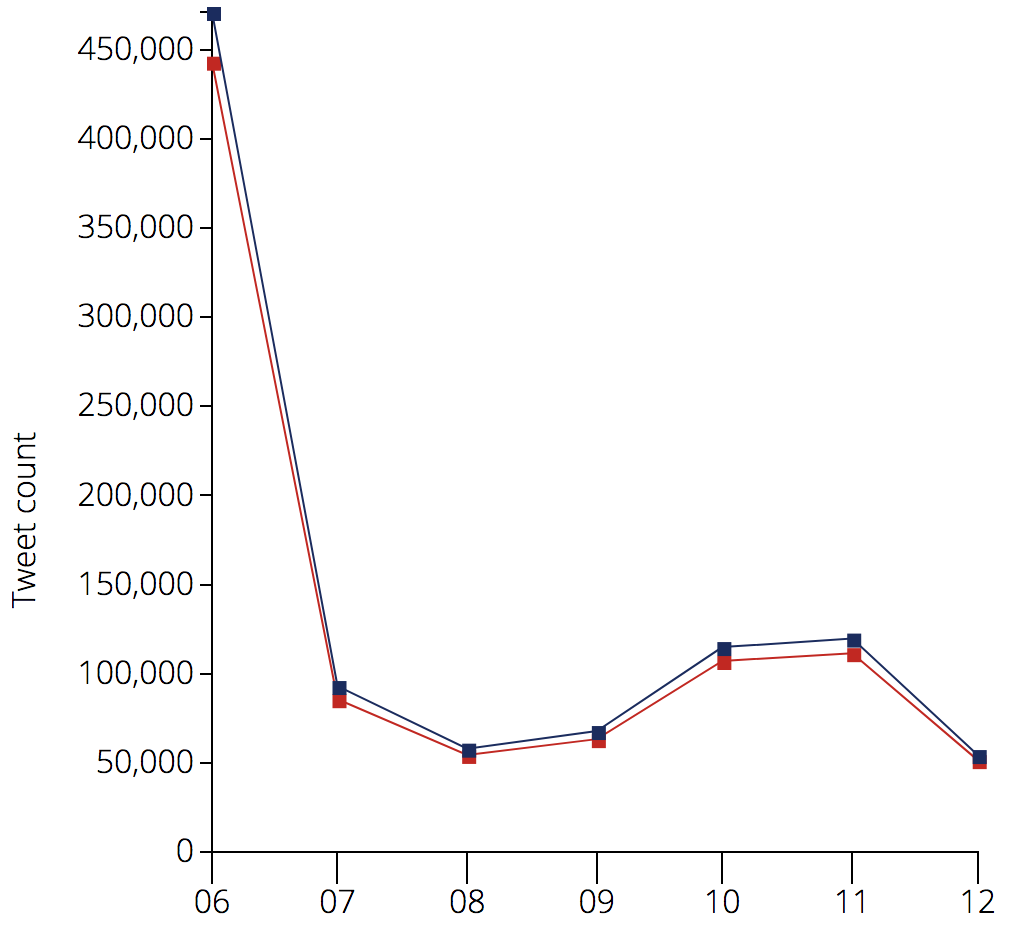
\includegraphics[width=\linewidth]{images/2016-brexit.png}
                \caption{2016}
                \label{fig:gull}
        \end{subfigure}%
        \begin{subfigure}[b]{0.33\textwidth}
                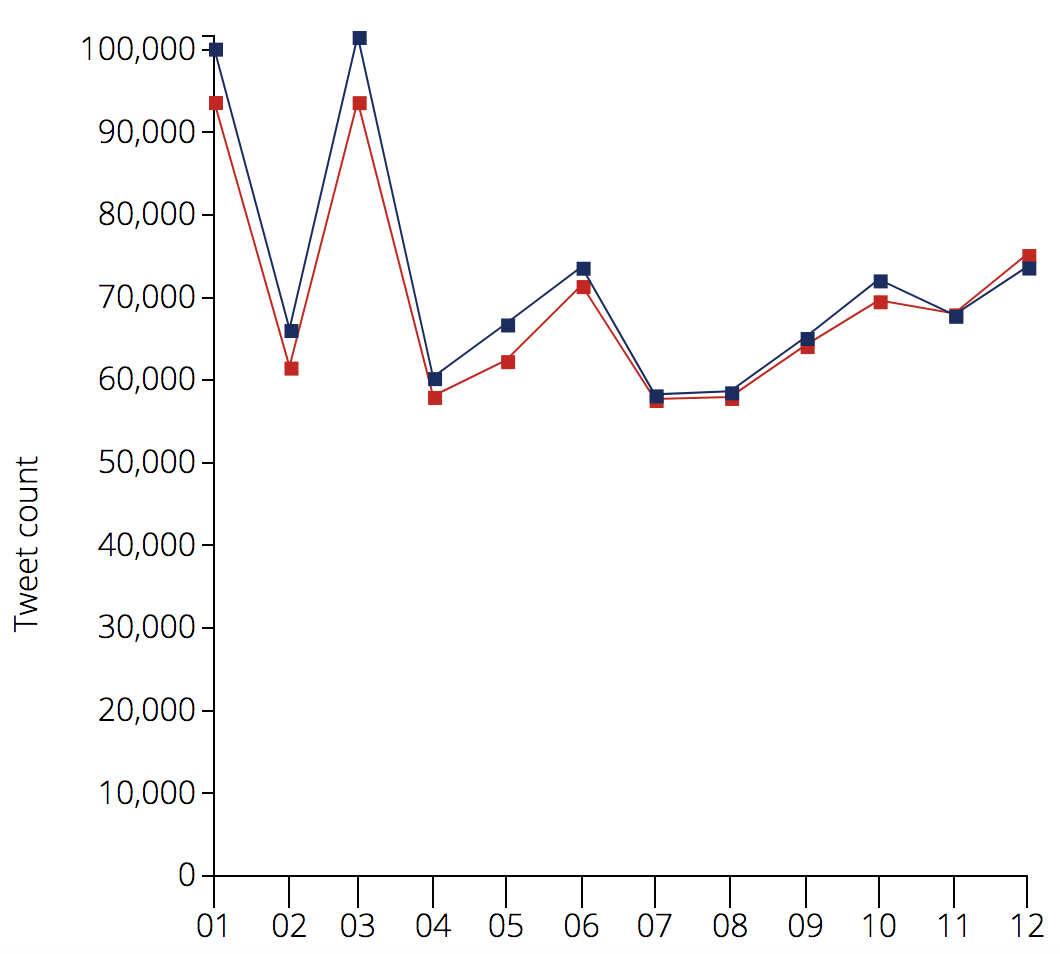
\includegraphics[width=\linewidth]{images/2017-brexit.png}
                \caption{2017}
                \label{fig:gull2}
        \end{subfigure}%
        \begin{subfigure}[b]{0.30\textwidth}
                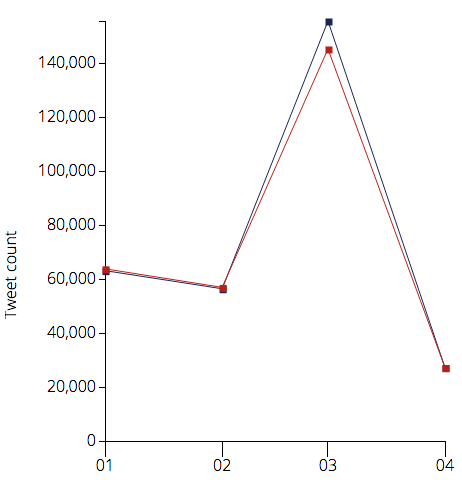
\includegraphics[width=\linewidth]{images/2018-brexit.png}
                \caption{2018}
                \label{fig:tiger}
        \end{subfigure}%

        \caption{Brexit Stance Model Results}\label{fig:brexit-results}
\end{figure}

\begin{figure}[H]
        \begin{subfigure}[b]{0.35\textwidth}
                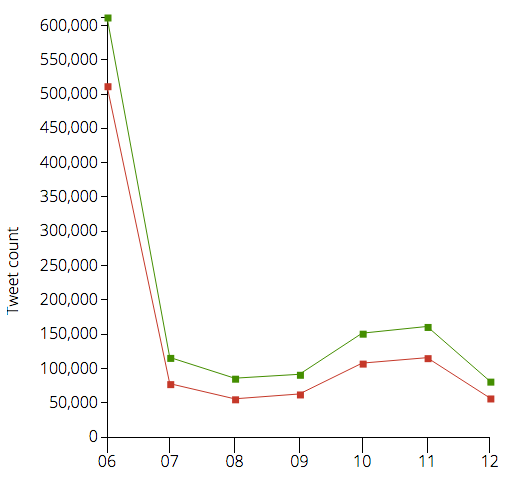
\includegraphics[width=\linewidth]{images/2016-sentiment.png}
                \caption{2016}
                \label{fig:gull}
        \end{subfigure}%
        \begin{subfigure}[b]{0.33\textwidth}
                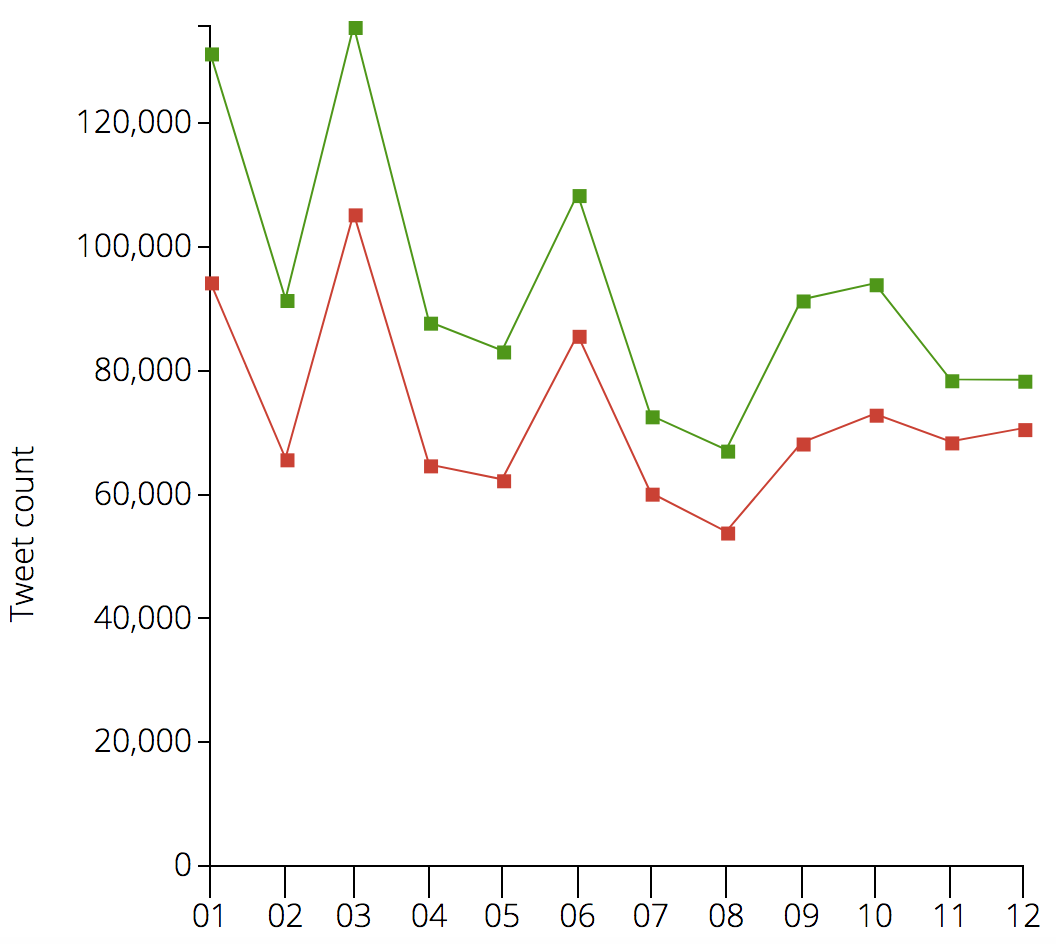
\includegraphics[width=\linewidth]{images/2017-sentiment.png}
                \caption{2017}
                \label{fig:gull2}
        \end{subfigure}%
        \begin{subfigure}[b]{0.30\textwidth}
                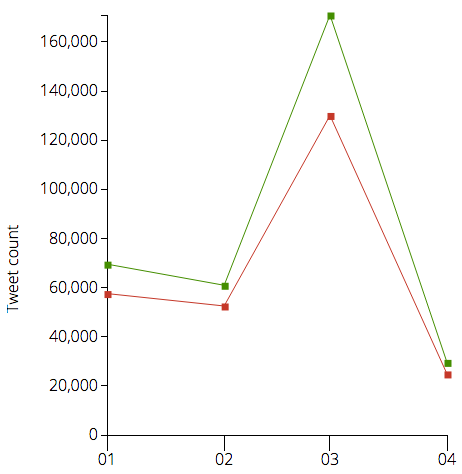
\includegraphics[width=\linewidth]{images/2018-sentiment.png}
                \caption{2018}
                \label{fig:tiger}
        \end{subfigure}%

        \caption{Sentiment Model Results}\label{fig:sentiment-results}
\end{figure}

\subsection*{Performance}
The System's two time consuming operations are the tokenization and classification of tweets. Through testing of the System on a computer with a 2.7 GHz Intel Core i5 dual core processor and three threads available to the System; it achieved 320 tokenizations per second and 280 classifications per second. On computers of a higher specification, the thread number could be higher and thus would result in a higher rate per second for both operations.


\subsection*{System Comparison}
The final System can be compared to the Brexit Systems mentioned within the related work. Table \ref{table:comparison} shows how the System developed within this report compares to the Edinburgh \citep{llewellyn_brexit?_2016} and Sheffield \citep{maynard_framework_2017} Systems. The results show that the System developed as part of this paper has incrementally improved on the current Systems that have analysed Brexit.

\begin{center}
\begin{tabular}{ |p{3cm}||p{2cm}|p{2cm}|p{2cm}|}
 \hline
 System & Real-Time & Machine Learning & Deep-Learning\\
 \hline
  Edinburgh & Yes & No & No \\
 \hline
 Sheffield & Yes & Yes & No \\
  \hline
 Our System & Yes & Yes & Yes \\
 \hline
\end{tabular}
\captionof{table}{System Comparison.}
\label{table:comparison}
\end{center}



\section{Future Work}
During the inception of the project there was scope to implement a variety of aspects to the real time sentiment analysis system. However, due to the time constraints of the project it was necessary to hone in on the detailed implementation of the System Features as identified within this report. This therefore leaves the below list of features that would provide ideal extensions to the system.

\begin{itemize}
\item Baseline Comparison: The System confidence in classification accuracy would benefit off of the implementation of a baseline accuracy through an SVM classifier rather than the existing comparison of a random distribution accuracy.

\item Online Learning: The Systems models were trained on small sample sizes due to the amount of data available at the time of training. As the System continuously collects tweets an extension would be to have the System retrain it's classification models when new training data becomes available thus learning in an online fashion.
 
\item Emotion Classification: As the System can easily integrate new classification models, predicting the Emotion of tweets could be added as a model. The model would classify tweets regarding Brexit using a six point mood scale \citep{pepe_between_2008} and would allow for the extraction of more analysis into sentiment on the issue. Thus as an extension the System could have a model which is classified on the distant labelling of emotions categories.
\end{itemize}

\end{document}